\section{Evaluation} \label{sec:evaluation}

Our evaluation used three Dell R430 servers as replicas. Each server having 
Linux 3.XX.X, 2.6 GHz Intel Xeon CPU with 24 hyperthreading cores, 32GB memory, 
and 1T SSD. Each machine has a Mellanox ConnectX-3 Pro Dual Port 40 Gbps NIC. 
These NIC are connected using the InfiniBand RDMA architecture through a Dell 
S6000 high-performance switch with 32 40Gpbs ports. The price of these 
RDMA-relevant hardware were moderate: each server costs US \$5,328 and the 
switch costs US \$12,894.

We evaluated \xxx on \nprog server programs, including \redis, 
\memcached, \ssdb, and \mongodb, \nkvprog key value stores; \mysql, a SQL 
server; \clamav, a anti-virus server that scans files and delete malicious 
ones; \mediatomb, a multimedia storage server that stores and transcodes video 
and audeo files; \openldap, a LDAP server, \tftp, a FTP server. In addition 
to these widely used \npopularprog programs, We have also evaluated \calvin, an 
advanced transactional database system that leverages \zookeeper as its SMR 
service. All these programs are multithreaded except \redis (but it can still 
serve requests concurrently using Libevent). These servers all process, 
update, and store important data and files, thus the high fault-tolerance of SMR 
is especially attractive to these programs.

\begin{table}[b]
\footnotesize
\centering
\vspace{-.05in}
\begin{tabular}{lrr}
{\bf Program} & {\bf Benchmark} & {\bf Benchmark workload description}\\
\hline\\[-2.3ex]
\clamav & Self  & Scan files in \v{/usr/lib} directory \\
\mediatomb & ApacheBench  & Transcode video files in parallel\\
\memcached & mcperf  & 50\% set and 50\% put operations\\
\mongodb & YCSB  & Workload C\\
\mysql & Sysbench  & Concurrent SQL transactions\\
\openldap & Self  & TBD\\
\redis & Self  & 50\% set and 50\% put operations\\
\ssdb & Self  & 50\% set and 50\% put operations\\
\calvin & Self  & Concurrent SQL transactions\\
\end{tabular}
\vspace{-.05in}
\caption{{\em Benchmarks and workloads.} ``Self" in the Benchmark column means 
we used a server program's own performance benchnmark.} 
\label{tab:benchmarks}
\end{table}


% Benchmarks table.
To evaluate the \xxx's practicality, we used popular third-party or the 
developers' own performance benchmarks for all these servers. For benchmark 
workload settings, we used the benchmarks' default workloads whenever 
available. Table~\ref{tab:benchmarks} introduces the benchmarks and workloads 
we used. To mitigate network latency of public network, all benchmarks were 
ran in a Dell R320 server, with Linux 3.XX.X, 2.2GHz Intel Xeon with 12 
hyperthreading cores, 16GB memory, and 160G SSD. This server connects with the 
replica machines with 1GBps 1Gbps bandwidth LAN, with a mean 401 \us ping 
round-trip latency. A larger latency (\eg, running clients from WAN) will 
further mask \xxx's overhead. We spawned up to 16 concurrent connections 
which made these servers reached peak throughput, and then we measured both 
response time (latency) and throughput. We also measured \xxx's bare 
latency on consensus. Each performance data point in the evaluation is taken 
from the mean value of 10 repeated executions.

% evaluation metric. client benchmarks all run in LAN, average latency



\subsection{Performance Overhead} \label{sec:overhead}

\begin{figure*}[t]
\centering
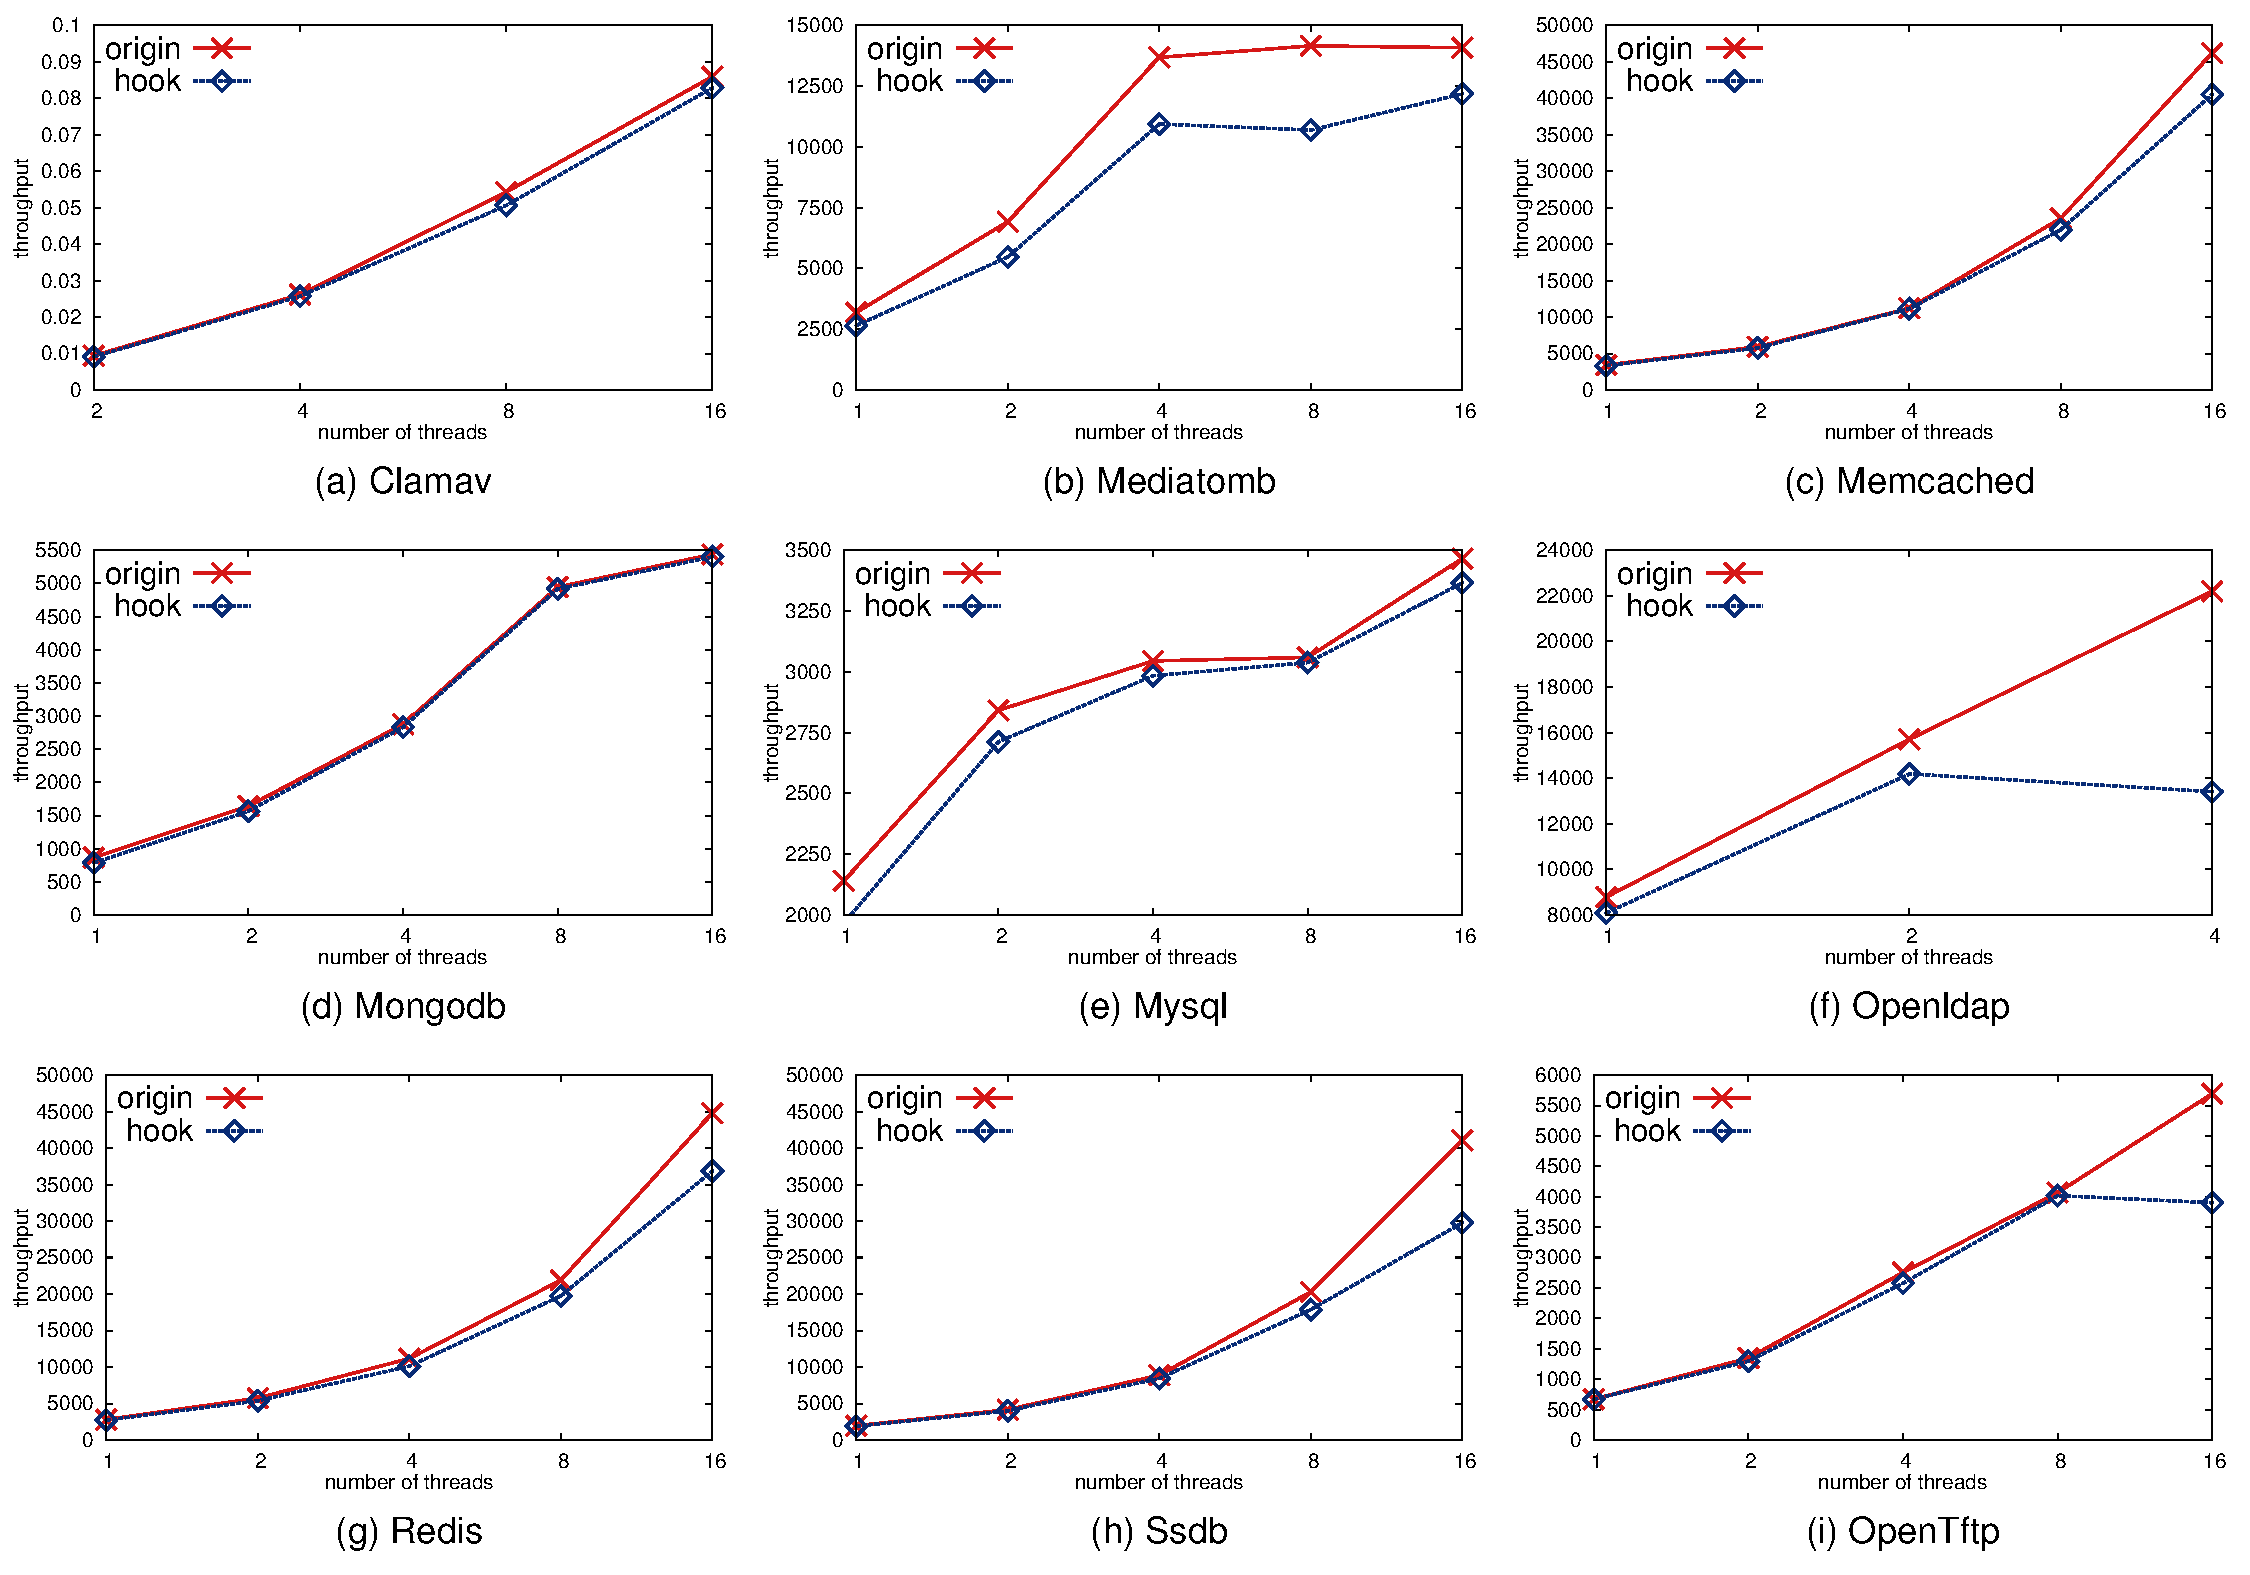
\includegraphics[width=0.9\textwidth]{figures/throughput}
\vspace{-.20in}
\caption{\small {\em \xxx throughput compared to the unreplicated 
execution.}}
\label{fig:tput}
\end{figure*}

\begin{figure}[t]
\centering
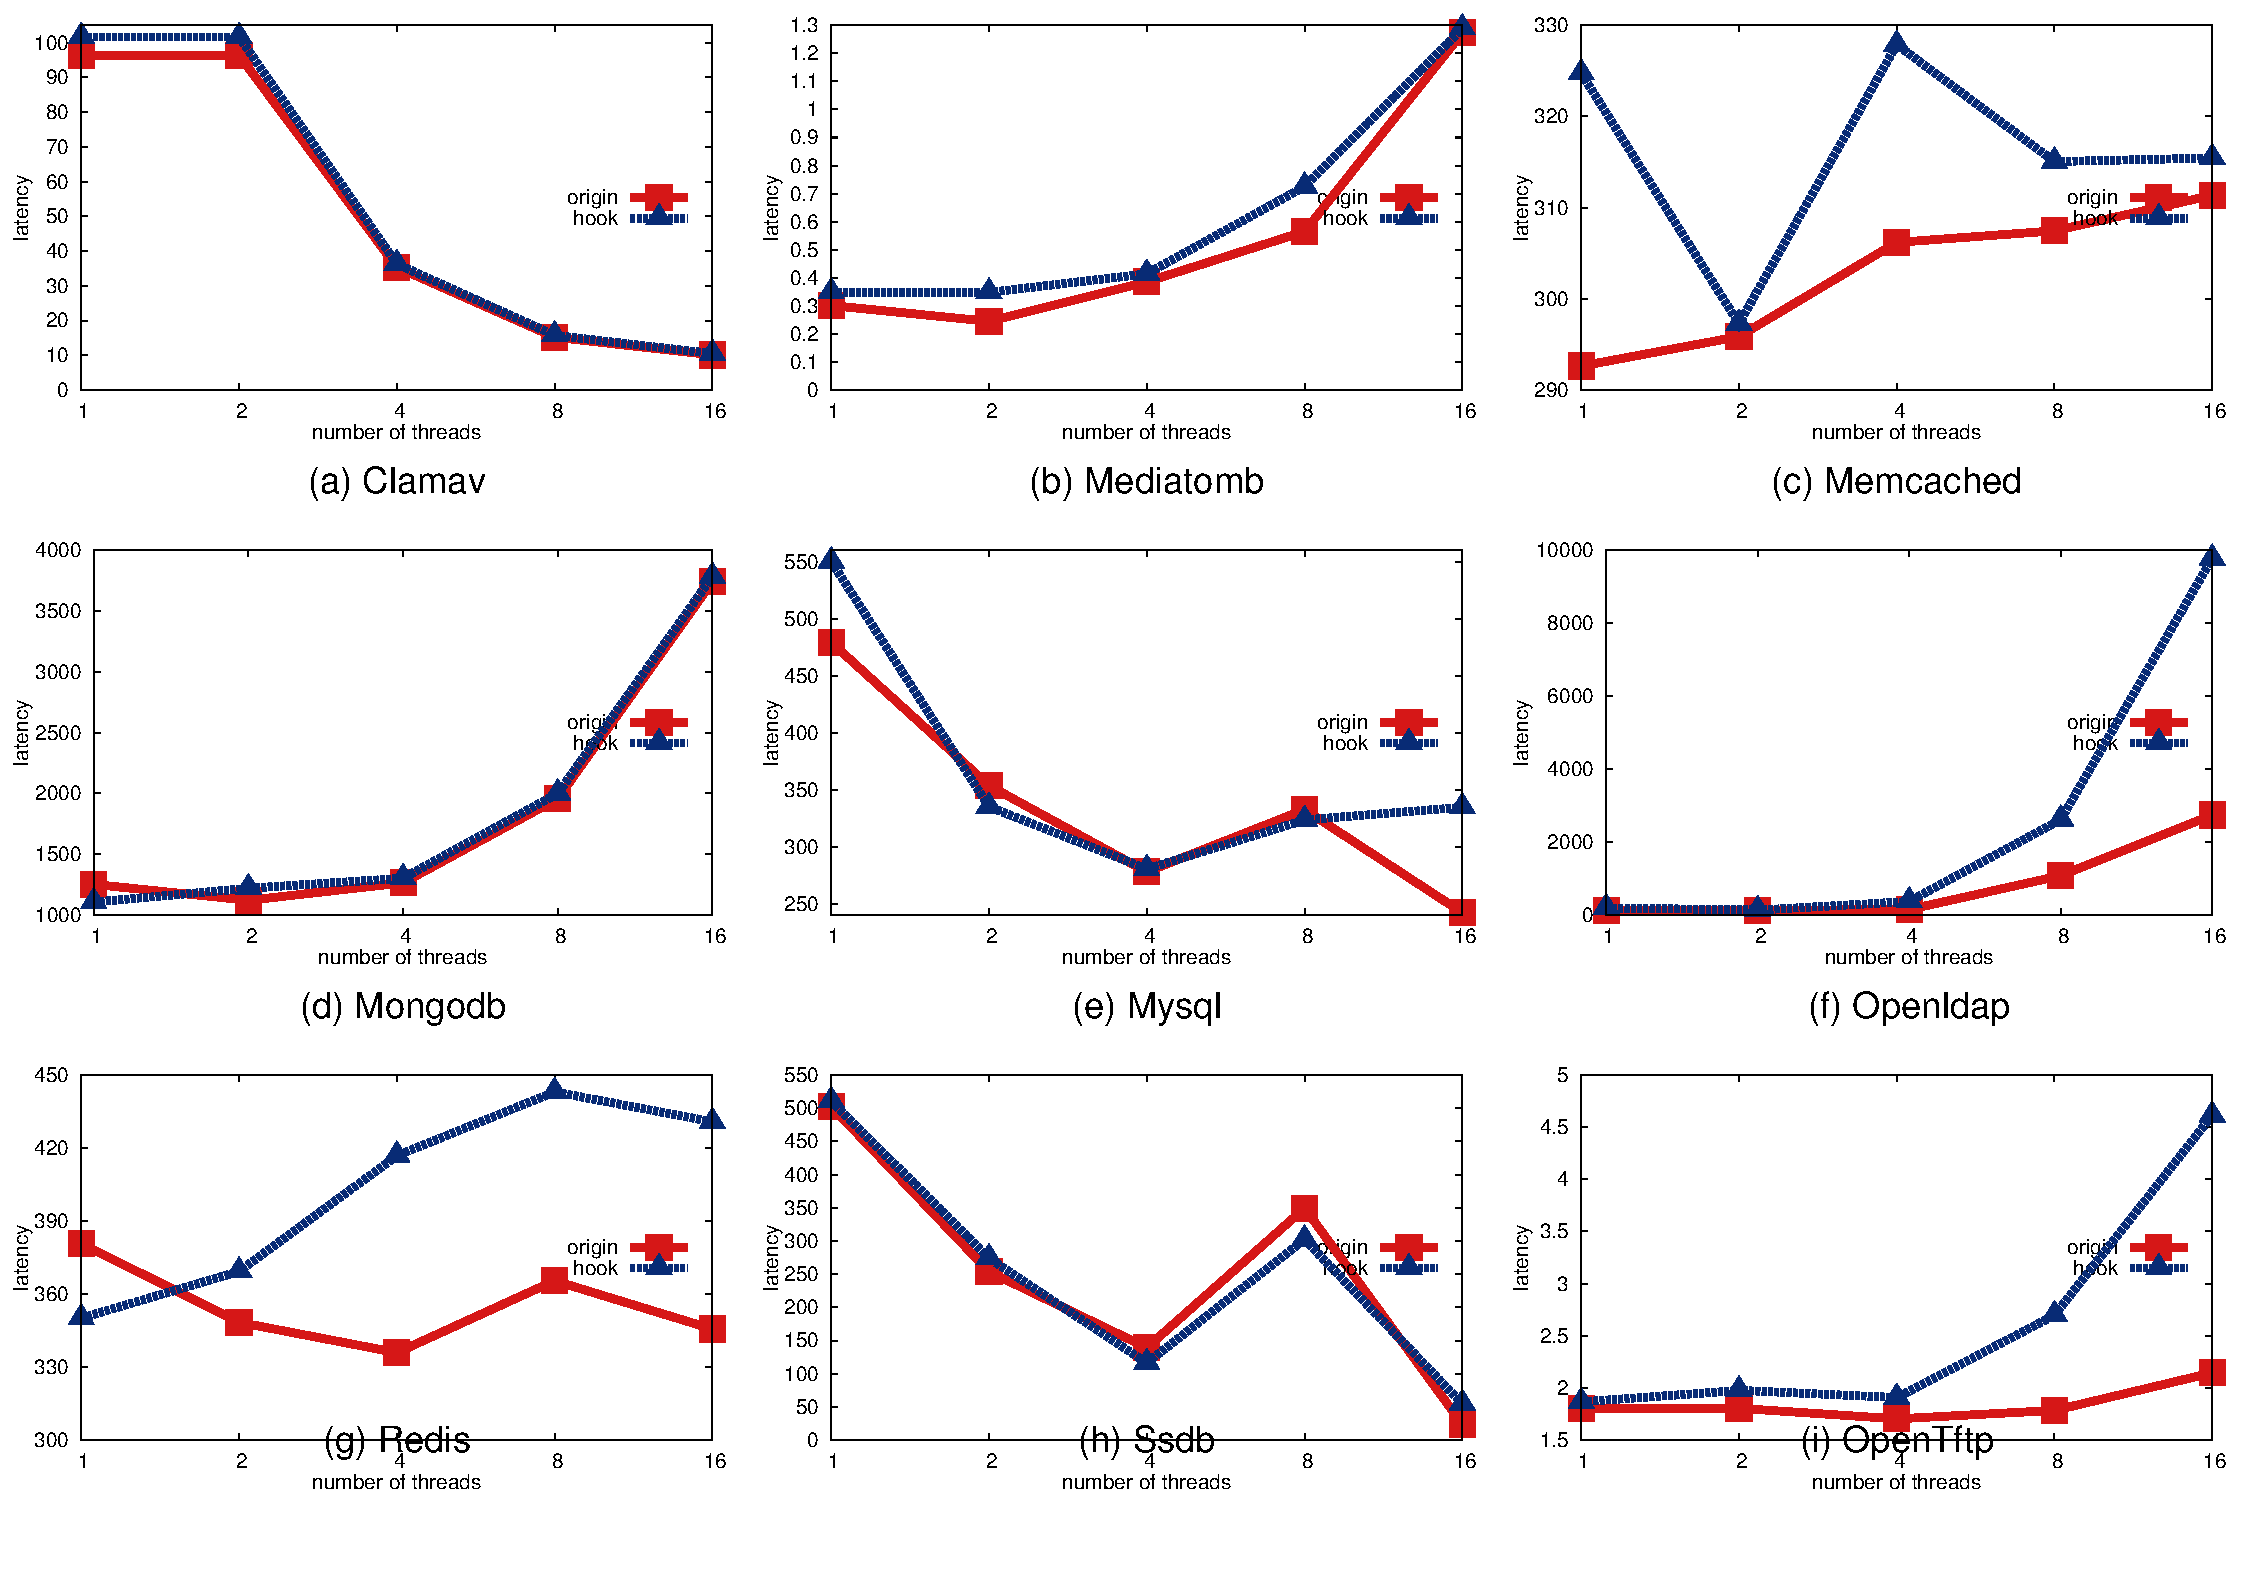
\includegraphics[width=0.9\textwidth]{figures/latency}
\vspace{-.20in}
\caption{\small {\em \xxx response time compared to the unreplicated 
execution.}}
\label{fig:latency}
\end{figure}

\begin{table}[b]
\footnotesize
\centering
\vspace{-.05in}
\begin{tabular}{lrrrrr}
{\bf Program} & {\bf \# calls} & {\bf input} & {\bf SSD} 
& {\bf quorum} & {\bf diff}\\
\hline\\[-2.3ex]
\clamav & 30  & 42.0 & 5.1 \us & 6.1 \us & F\\
\mediatomb & 3,000  & 140.0 & 4.7 \us & 5.8 \us & F?\\
\memcached & 10,016  & 38.0 & 4.9 \us & 6.9 \us & F?\\
\mongodb & 25,665  & 492.4 & 19.1 \us & 20.4 \us & F?\\
\mysql & 13,111  & 26.0 & 5.0 \us & 15.7 \us & W?\\
\openldap & 8,040  & 27.3 & 5.7 \us & 7.1 \us & T\\
\redis & 10,016  & 107.0 & 3.6 \us & 6.3 \us & T\\
\ssdb & 9,916  & 47.0 & 3.7 \us & 10.9 \us & F*\\
\calvin & TBD  & TBD & TBD  & TBD & TBD\\
\end{tabular}
\vspace{-.05in}
\caption{{\em \xxx micro events.} The ``\# Calls" column means the number of 
socket calls that went through \xxx input concensus; ``input" means average 
bytes of a server's inputs received in these calls; ``SSD" means the average 
latency on storing these calls to stable storage; ``quorum" means the
average latency on waiting quorum for these calls; and ``diff" means whether 
the 
output checker found output divergence.} 
\label{tab:consensus-latency}
\end{table}


TBD.
% Overhead compared with unreplicated executions.

TBD.
% Bare consensus latency, micro events.

\subsection{Scalability on Replica Group Size} \label{sec:scalability}

TBD.
% 3, 5.

\subsection{Comparison with Traditional SMR systems} \label{sec:compare}

TBD.
% Run Calvin on Zookeeper, Crane, and Falcon. Because we can only make Calvin's 
% database with Zookeeper. XX speedup.

\subsection{Recovering from Output Divergence} \label{sec:robust}

TBD.
% Change 

\subsection{Sensitivity of Parameters} \label{sec:sensitivity}

% Change output comparison periods. 1, 100, 1000, 10000. 1000 is the smallest 
% number that starts to have negligible overhead. Run only with the server with 
% largest recv() data size.

% Twait

% Tcomphash
 
% \subsection{Read-only Optimization} \label{sec:read-opt}

% % 